\subsection*{Question 4}

\noindent Before using OClover, we first need to modify \textit{pom.xml} file in order to add the plugin to the project. In order to do so, we add the following lines in the \textit{plugin} section of the \textit{pluginManagement} section of the \textit{pom.xml} file.

\begin{center}
        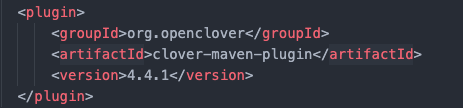
\includegraphics[width=0.8\textwidth]{img/cloverxml.png}
\end{center}
\noindent Using the terminal, from within the project folder, the command
\begin{verbatim}
    mvn clean clover:setup test clover:aggregate clover:clover
\end{verbatim}
\noindent will run the code coverage tool on the project and generate a report as for JaCoCo. The reports can be found in the target \verb|../target/site/clover/| folder accessible as an .html or .xml file.\\
\noindent The \textit{pom.xml} file used to run OClover tool on this project is joined with the report as \textit{q4.xml}.
